\subsection{Reorganization following removal or addition of neurons}

The final and most challenging experiment is to test how the RSOM can cope
with degenerative cases, where either neurons die out (removal) or new units are added to the map (addition). Figure~\ref{fig:reorganization:results}A illustrates an example of a well-formed neural space (black outlined discs), a removal (red disks) and an addition (black dots). For both removal and addition, we applied a LLoyd relaxation scheme to achieve a new quasi-centroidal Voronoi tesselation. Figures \ref{fig:reorganization:results}B and \ref{fig:reorganization:results}C depicts the Voronoi tesselations after $100$ iterations starting from the initial tesselation shown in panel \ref{fig:reorganization:results}A. 

In order to conserve as much as possible the original topology, we used a differentiated procedure depending on if we are dealing with a removal or an addition. In case of removal, only the remaining neurons that were previously connected to a removed unit are allowed to connect to a new unit unconditionally. For the rest of the units, they might reconnect to a nearby unit if this unit is much closer than its closest current neighbour (85\% of the smallest distance to its current neighbours). In case of addition, new units can connect unconditionally to the nearest neighbours while old unit can only connect to the newly added unit if this unit is much closer than its current closest neighbour (85\% of the smallest distance to its current neighbours). This procedure guarantees that the topology is approximately conserved as shown in figures \ref{fig:reorganization:results}D-F. We tested the alternative of recomputing the graph from scratch but the resulting topology is quite different from the original because of micro-displacements of every units following the Lloyd relaxation.

Learning is performed in two steps. First we iterate $25,000$ epochs using the intact map, then we perform removal and addition and learning is iterated for another $5,000$ epochs for all three maps (orginal map, map with added units and map with removed units). The final self-organization is shown in figures \ref{fig:reorganization:results}G-I where we can observe strong similarities in the organization. For example, the central red patch is conserved in all three maps and the overall structure is visually similar. Of course, these results depend on the number of removed or added units (that needs to be relatively small compared to the size of the whole map) and their spatial distribution.
%\gid{the last two paragraphs are not too clear, they seem confusing}

%\gid{TODO Add a few more words here. Maybe make a connection to neuroscience facts about reorganization.} \npr{maybe in the discussion instead} \gid{Agreed} \nrp{Done}.

%Previous studies have shown that after an ablation or addition of units the map undergoes a reorganization of its neural representations. The immediate  consequence of a reorganization is the acquisition of new receptive fields. When an ablation takes place, unaffected neurons try to recover representations that got lost due to neurons death. In addition, on the other hand, the surplus neurons have to get their share of the representations and thus the entire map undergoes a reorganization.

%The induced topology shares similarity with the original topology (before ablation or addition). 

% It is known that this sort of reorganization takes place naturally within brain. More precisely, neurogenesis happens in the subgranular zone of the Dentate Gyrus (DG) of the hippocampus and in the subventricular zone of the lateral ventricle~\cite{Alvarez:2004}. On the other hand, when neural tissue in the cerebral cortex~\cite{Merzenich:1984,Taub:2014} or the spinal cord~\cite{Bareyre:2004,Liu:1958}, the undamaged neurons reorganize their receptive fields and undamaged nerves sprout new connections, respectively, partially or fully restore functionality. Therefore, the study of reorganization after a neural ablation or neurogenesis within a self-organizing map is detrimental. 


\begin{figure}
  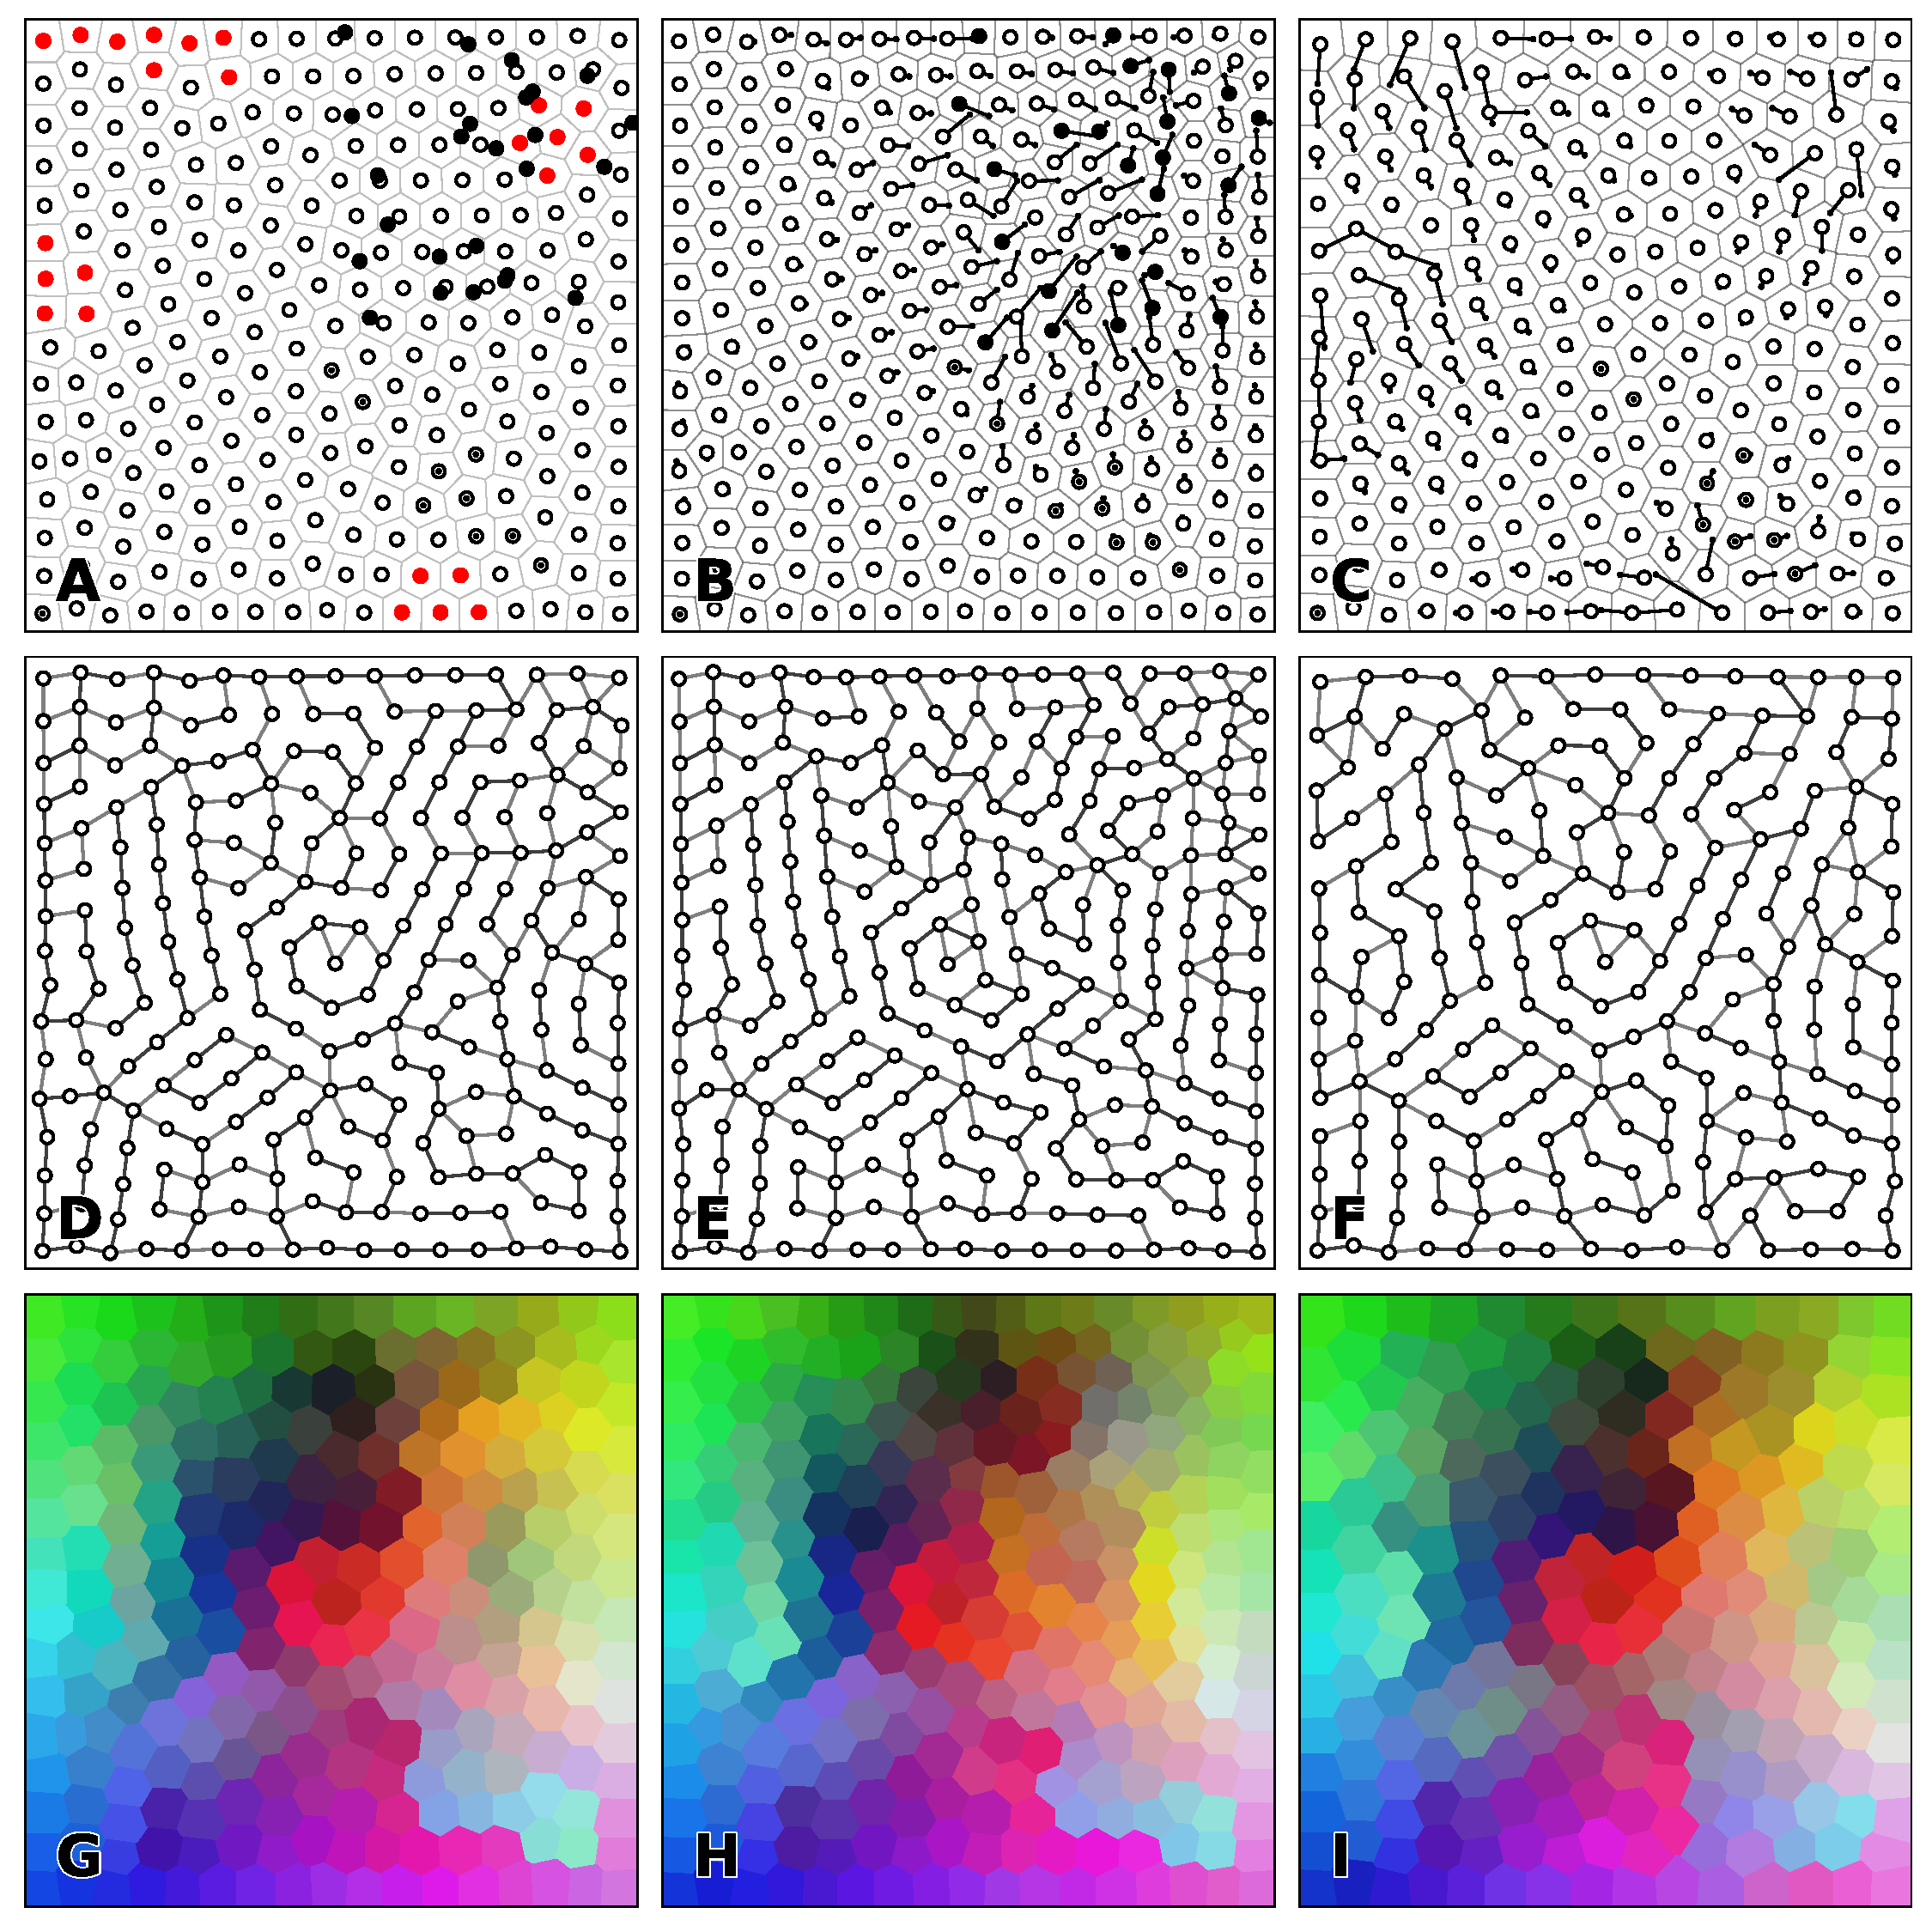
\includegraphics[width=\columnwidth]{experiment-reorganization.pdf}
  \caption{%
  {\bfseries \sffamily Reorganization (results).}
  %
  An initial set of 248 neurons (outlined discs on panel \textbf{A}) has been modified with the addition of 25 neurons (black discs) or the removal of 25 neurons (red discs). Panels \textbf{B} and \textbf{C} show the final position of neurons after 100 iterations of the centroidal Voronoi tesselation. Lines shows individual movement of neurons. Panels \textbf{D}, \textbf{E} and \textbf{F} show the 2-neighbors induced topology for \textbf{A}, \textbf{B} and \textbf{C} respectively. Panels \textbf{G}, \textbf{H} and \textbf{I} show the map
  map codebook for each map in neural space after learnin. Each voronoi cell of a neuron is painted with the color of the related codeword.
  %
  }
  \label{fig:reorganization:results}
\end{figure}
